\documentclass[10pt, notes]{beamer}

\usetheme[background=dark, numbering=fraction]{metropolis}
\usepackage{appendixnumberbeamer}
\usepackage{color, xcolor}
\usepackage{dsfont}
\definecolor{mydarkblue}{rgb}{0,0.08,0.45}


\usepackage{booktabs}
\usepackage[scale=2]{ccicons}


\usepackage{adjustbox} 
\usepackage{pgfplots}
\usepgfplotslibrary{dateplot}
\usepackage{fourier-orns}
\usepackage{xspace}

\usepackage[scale=2]{ccicons}
\usepackage{fontawesome}


\usepackage[backend=bibtex,style=authoryear]{biblatex}
\addbibresource{index.bib}
\renewcommand*{\bibfont}{\scriptsize}



\newcommand{\themename}{\textbf{\textsc{metropolis}}\xspace}
% \DeclareMathOperator*{\argmin}{arg\,min}
% \DeclareMathOperator*{\minimize}{minimize}
% \DeclareMathOperator*{\maximize}{maximize}

\makeatletter
\renewcommand{\metropolis@colors@dark}{%
  \setbeamercolor{normal text}{%
    fg=black!2,
    bg=mDarkTeal
  }%
  \usebeamercolor[fg]{normal text}%
}
\renewcommand{\metropolis@colors@light}{%
  \setbeamercolor{normal text}{%
    fg=mDarkTeal,
    bg=black!2
  }%
  \usebeamercolor[fg]{normal text}%
}
\makeatother

\usepackage{tikz}
\usetikzlibrary{matrix,chains,positioning,decorations.pathreplacing,arrows}


\title{\huge Parallel Optimization and Machine Learning}
\author{
\large{\bfseries Fabian Pedregosa}}
% {\normalsize{ includes work with Remi Leblond and Simon Lacoste-Julien}}}
% \author{
% \hspace{4.8em}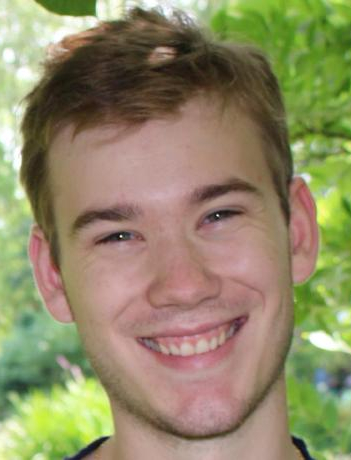
\includegraphics[width=0.2\linewidth]{img/remi}
% \hspace{4.8em}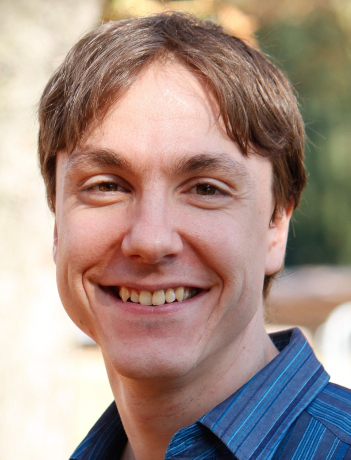
\includegraphics[width=0.2\linewidth]{img/SLJ}
% }\\
% {\normalsize\vphantom{}\hspace{0.5em} Fabian Pedregosa \hspace{3.5em} R\'emi Leblond \hspace{2.2em} Simon Lacoste--Julien}\\
% \vphantom{}\\
% \vphantom{}
\includegraphics[width=0.3\linewidth]{img/logo_inria}
% 
\includegraphics[width=0.12\linewidth]{img/ens.png}
% \hspace{0.5em}
\includegraphics[width=0.3\linewidth]{img/montreal}
% \hspace{0.5em}
\includegraphics[width=0.2\linewidth]{img/mila}
% }
% 
\institute{

{\centerline{\hspace{2em}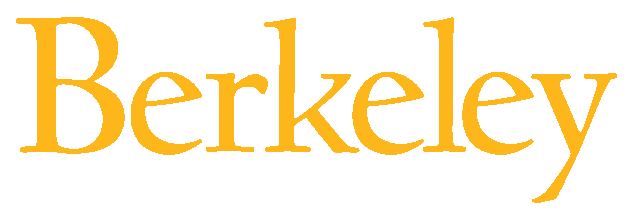
\includegraphics[width=0.3\linewidth]{img/Berkeley_wordmark_gold_no_uc}\hspace*{2em}

\includegraphics[width=0.3\linewidth]{img/eth_logo_kurz_neg}\hspace*{2em}
{
\includegraphics[width=0.25\linewidth]{img/eu}}
}}
}
%\titlegraphic{\hfill\includegraphics[height=1.5cm]{figures/UCBerkeley_wordmark_blue.eps}}
\date{\vspace{1em}\today~{Huawei Paris Research Center}}

\input defs.tex



\begin{document}

\maketitle

\metroset{background=light} % change background theme according to manual
{
\usebackgroundtemplate{%
\begin{picture}(40,260)
  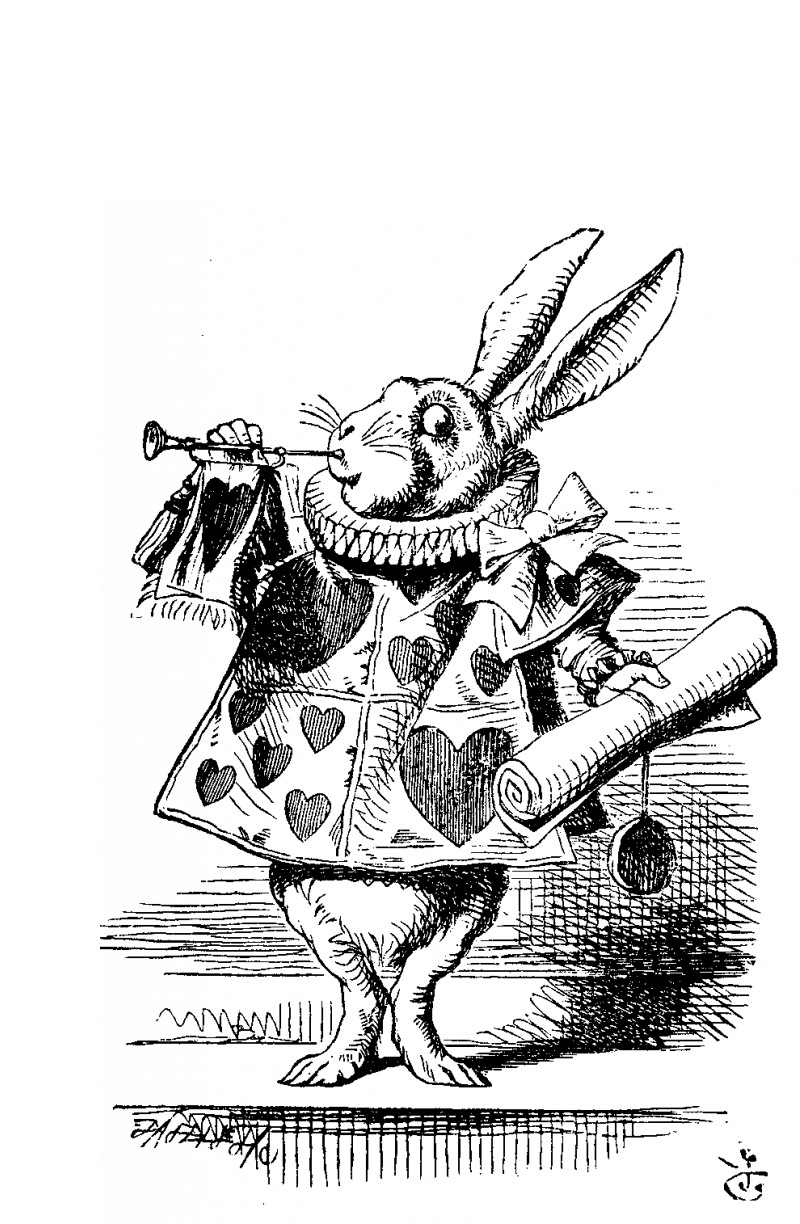
\includegraphics[height=0.9\paperheight]{img/white-rabbit}
  \end{picture}
  }
\begin{frame}{About me}
\begin{columns}
\begin{column}{0.4\textwidth}  %%<--- here
\end{column}
\begin{column}{0.6\textwidth}  %%<--- here
\begin{itemize}
\item Engineer (2010-2012), Inria Saclay.
\item PhD (2012-2015, Inria Saclay)
\item Postdoc (2015-2016), Dauphine--ENS--Inria Paris.
\item Postdoc (2017-present), UC Berkeley - ETH Zurich (Marie-Curie fellowship, European Commission)
\end{itemize}
\end{column}
\end{columns}

\note{I should start by presenting myself. I started my career as an engineer }

\end{frame}
}

\metroset{background=dark} % change background theme according to manual

\begin{frame}{Motivation}
\begin{columns}[T] % align columns
\begin{column}{.5\textwidth}
\centering{Computer add in 1993}
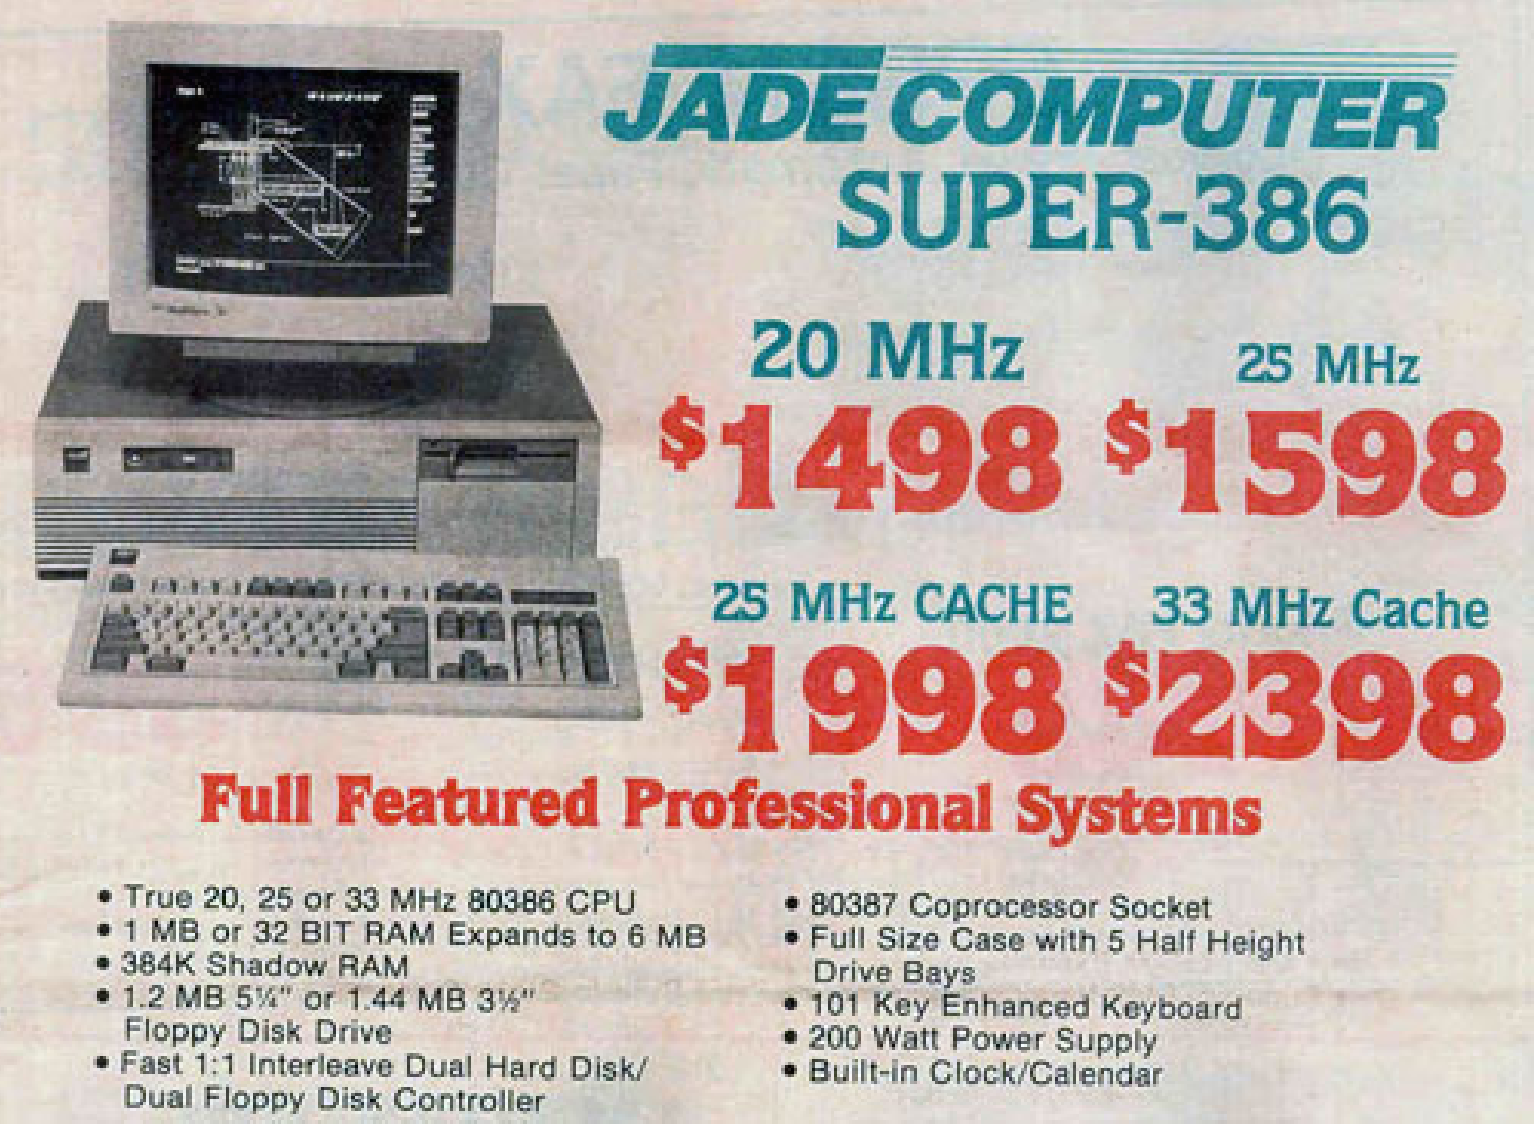
\includegraphics[width=1.05\linewidth]{img/old_ad}
\end{column}%
\hfill%
\begin{column}{.5\textwidth}
\centering{Computer add in 2006}
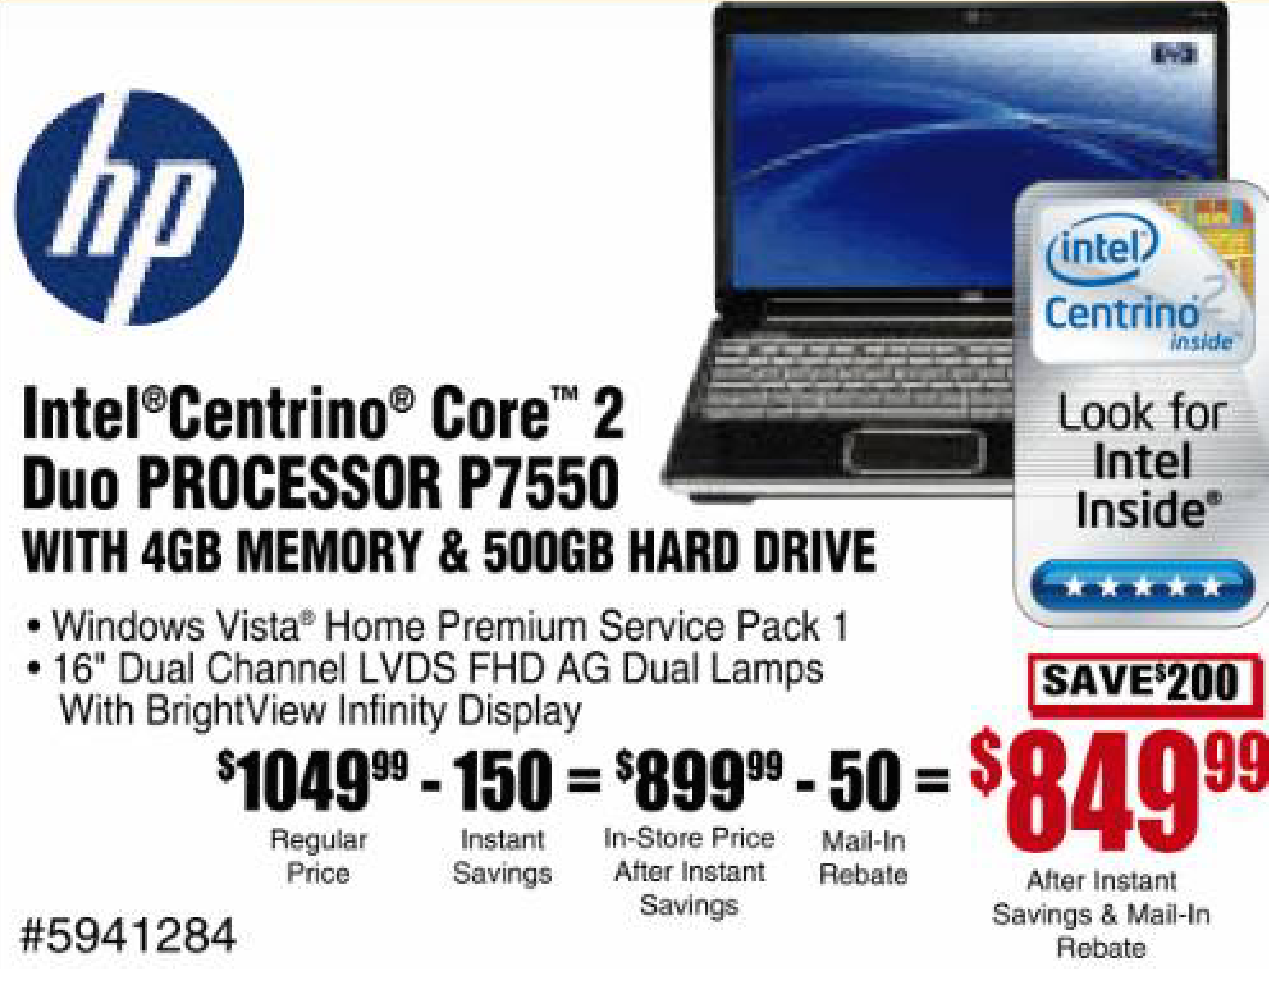
\includegraphics[width=\linewidth]{img/2006_ad}
\end{column}%
\end{columns}
What has changed?
\pause
2006 = no longer mentions to speed of processors
\end{frame}


\begin{frame}{Moore's law}
\begin{quote}
The complexity for minimum component costs 
has increased at a rate of roughly a factor of 
two per year. Certainly over the short term this 
rate can be expected to continue
\end{quote}
Gordon Moore (Intel), 1965

\hspace{1em}\begin{quote}
OK, maybe a factor of two every two 
years.
\end{quote}
Gordon Moore (Intel), 1975 [paraphrased]
\end{frame}


\begin{frame}{40 years of CPU trends}
\centering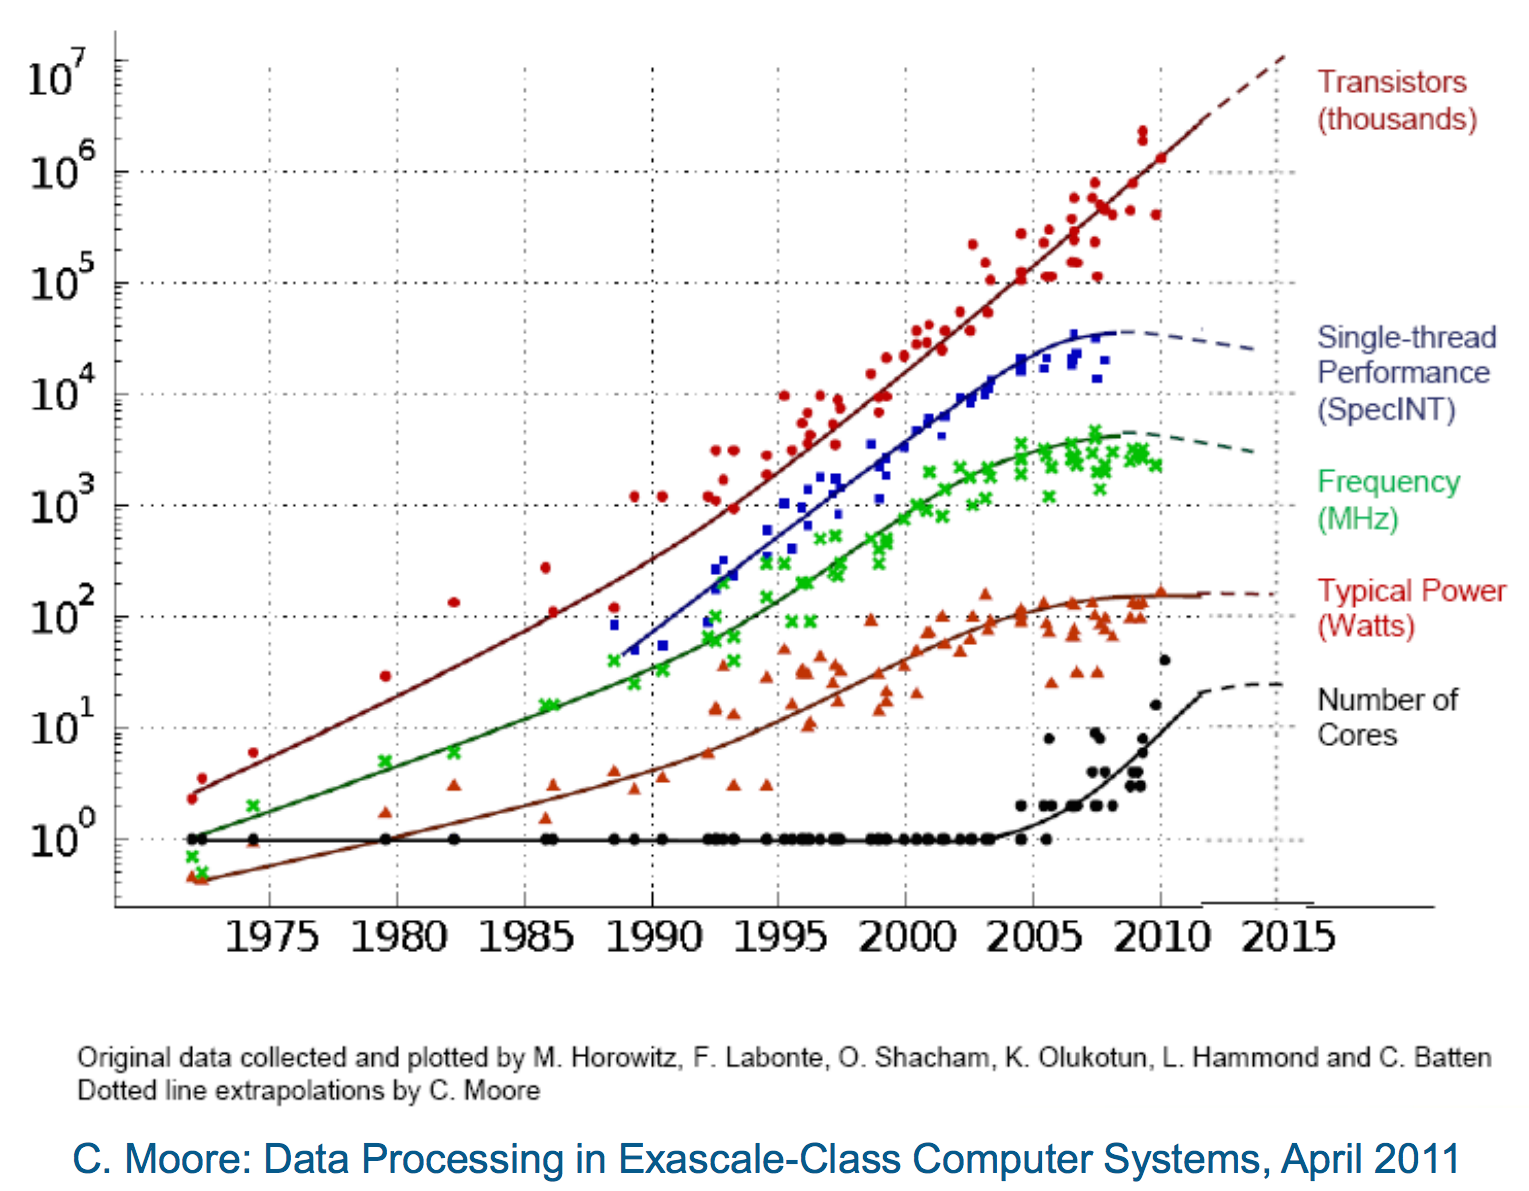
\includegraphics[width=0.8\linewidth]{img/moore_law}

\begin{itemize}[<+->]
\item Speed of CPUs has stagnated since 2005;
\item Multi-core architectures are here to stay.
\end{itemize}
\pause {\bfseries Parallel algorithms needed to take advantage of modern CPUs.}
\end{frame}


\begin{frame}{Outline}

{\bfseries Goal of the talk:} overview and state of the art in parallel optimization methods in machine learning.

\medskip

\begin{columns}[T] % align columns
\begin{column}{.5\textwidth}
{\centering \bfseries Synchronous methods}
\begin{itemize}
\item MapReduce (and variants: Hadoop, Spark)
\item ADMM
\item COCOA
\end{itemize}
\end{column}%
\hfill%
\begin{column}{.5\textwidth}
{\centering \bfseries Asynchronous methods}
\begin{itemize}
\item Asynchronous SGD
\item Variance-reduced methods
\end{itemize}
\end{column}%
\end{columns}
\vspace{1em}

Along the way, analysis of algorithms, our recent work.

\end{frame}

\begin{frame}{Outline}
Parallel algorithms can be divided  large categories: 
synchronous and asynchronous methods.

\begin{figure}
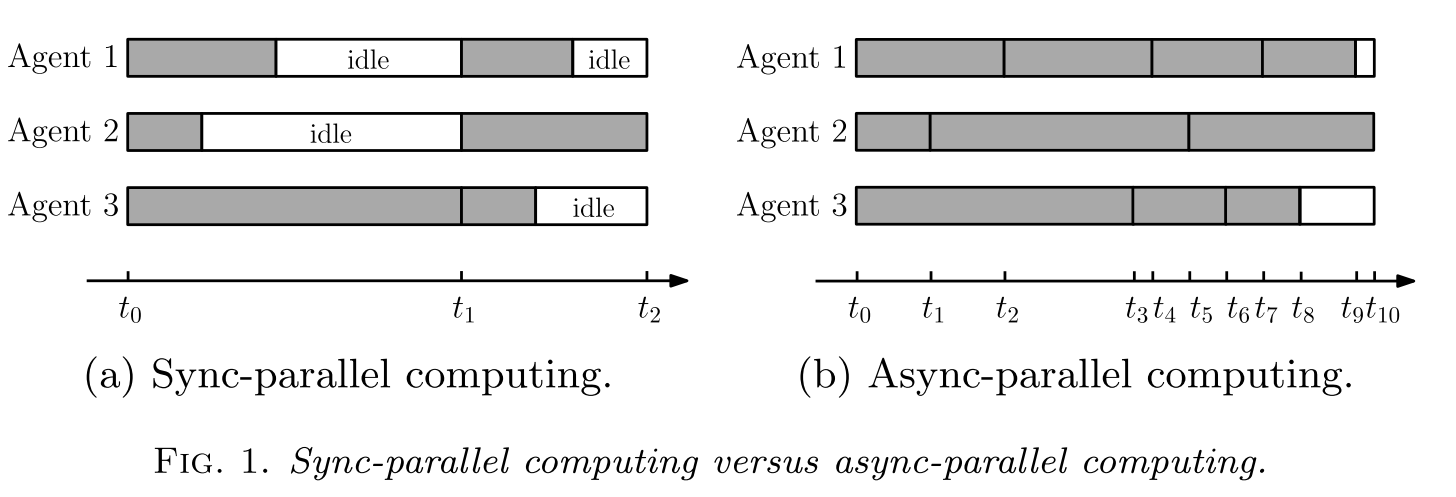
\includegraphics[width=\linewidth]{img/sync_vs_async}
{\small Image credits: \parencite{peng2016arock}}
\end{figure}
\end{frame}


\begin{frame}{Supervised Machine Learning}

{\bfseries Data}: $n$ observations $(\boldsymbol{a}_i, b_i) \in \mathbb{R}^p \times \mathbb{R}$

{\bfseries Prediction function}: $h(\boldsymbol{a}, \boldsymbol{x}) \in \RR$


{\bfseries Motivating examples:}
\begin{itemize}
\item Linear prediction: $h(\boldsymbol{a}, \xx) = \xx^T\boldsymbol{a}$
\item Neural networks: $h(\boldsymbol{a}, \xx) = \xx_m^T \sigma(\xx_{m-1}\cdots)$
\end{itemize}

\only<1>{
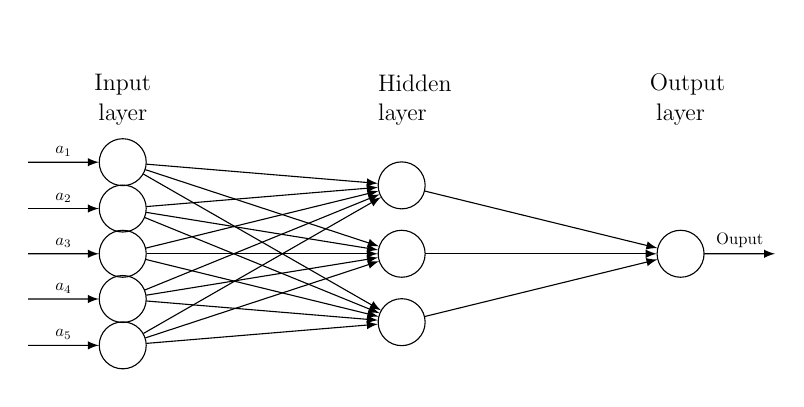
\begin{tikzpicture}[
ampersand replacement=\&,
scale=0.6,
every node/.style={scale=0.6},
plain/.style={
  draw=none,
  fill=none,
  },
net/.style={
  matrix of nodes,
  nodes={
    draw,
    circle,
    inner sep=10pt
    },
  nodes in empty cells,
  column sep=2cm,
  row sep=-9pt
  },
>=latex
]
\matrix[net] (mat)
{
|[plain]| \parbox{1.3cm}{\centering \Large Input\\layer} \& |[plain]| \parbox{1.0cm}{\centering\Large Hidden\\layer} \& |[plain]| \parbox{1.3cm}{\centering \Large Output\\layer} \\
\& |[plain]| \\
|[plain]| \& \\
\& |[plain]| \\
  |[plain]| \& |[plain]| \\
\& \& \\
  |[plain]| \& |[plain]| \\
\& |[plain]| \\
  |[plain]| \& \\
\& |[plain]| \\    };
\foreach \ai [count=\mi ]in {2,4,...,10}
  \draw[<-] (mat-\ai-1) -- node[above] {$\boldsymbol{a}_{\mi}$} +(-2cm,0);
\foreach \ai in {2,4,...,10}
{\foreach \aii in {3,6,9}
  \draw[->] (mat-\ai-1) -- (mat-\aii-2);
}
\foreach \ai in {3,6,9}
  \draw[->] (mat-\ai-2) -- (mat-6-3);
\draw[->] (mat-6-3) -- node[above] {Ouput} +(2cm,0);
\end{tikzpicture}
}
\only<2>{
{\bfseries Minimize some distance (e.g., quadratic) between the prediction}
$$
\minimize_{\xx} \frac{1}{n}\sum_{i=1}^n \ell(\boldsymbol{b}_i, h(\boldsymbol{a}_i, \xx)) \stackrel{\text{notation}}{=} \frac{1}{n}\sum_{i=1}^n f_i(\xx)
$$
}



\note{
The kind of parallelization will depend on the problem.
The kind of problem that we will be interested in
The problem: supervised learning.
}


\end{frame}


\begin{frame}{Optimization for machine learning}
\begin{center}
{ Minimize $F(x) = \displaystyle\frac{1}{n}\sum^{n}_{i=1} f_i(x)$}
\end{center}

\begin{columns}
\begin{column}{0.5\textwidth}  %%<--- here
{\bfseries Gradient descent} [Cauchy, 1847]: descend along $-\nabla F'(x)$

Updates of the form $$x^+ = x - \gamma \nabla F'(x)$$



{\bfseries Stochastic gradient descent} (SGD) [Robbins and Monro, 1951]: select a random index $i$ and descent along $~\nabla f_i(x)$,

Updates of the form $$x^+ = x - \gamma \nabla f_i(x)$$

\end{column}
\begin{column}{0.5\textwidth}  %%<--- here
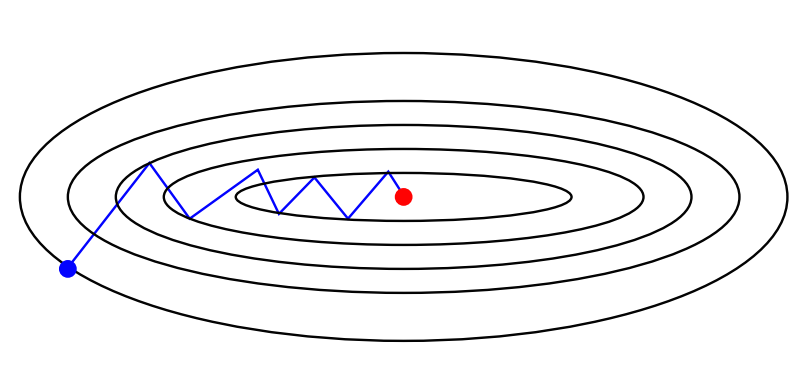
\includegraphics[width=\linewidth]{img/gd}

\vspace{2em}
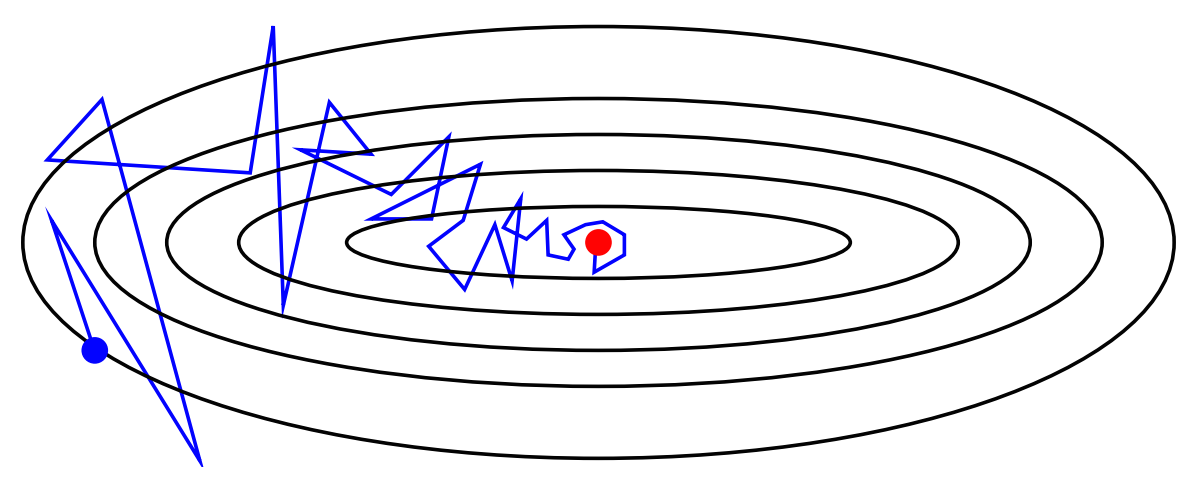
\includegraphics[width=\linewidth]{img/sgd}

\end{column}
\end{columns}







Images source: Francis Bach

\end{frame}




\begin{frame}{Composite objective}

\faExclamationTriangle~These methods assume objective function is smooth

Cannot be applied to Lasso, Group Lasso, box constraints, etc.

\pause 
\vspace{5mm}
{\bfseries Objective}: minimize composite objective function:
$$
\minimize_{\xx} f(\xx) + h(\xx)~,~ \text{ with $f(x) = \textstyle \frac{1}{n}\sum_{i=1}^n f_i(\xx)$}
$$
where $f_i$ is smooth and $h$ is a block-separable (i.e., $h(\boldsymbol{x}) = \sum_{B} h([\boldsymbol{x}]_B)$) convex function for which we have access to its proximal operator.
\end{frame}



% \begin{frame}{Sparse Proximal SAGA}
% 
% {\bfseries Contribution 1: Sparse Proximal SAGA.} Variant of SAGA \parencite{defazio2014saga}, particularly efficient when $\nabla f_i$ are sparse.
% % \vspace{0.5em}\begin{equation*}\tag{SAGA}
% % \xx^+ = \prox_{\gamma h}(\xx - \gamma (\nabla f_i(\xx) - \balpha_i + \overline{\balpha}))\,;~\balpha_i^+ = \nabla f_i(\xx)~.
% % \end{equation*}
% 
% % \begin{align}
% %     \vphantom{\sum}\vv_i &= \nabla f_i(\xx) - \balpha_i + \tikzmarkin<2>{a}\DD_i\tikzmarkend{a} \overline{\balpha}\,\\
% %     \vphantom{\sum}\xx^+ &= \prox_{\gamma \varphi_i}\big(\xx - \gamma \vv_i \big)\,;~
% %     \balpha_i^+ = \nabla f_i(\xx)
% % \end{align}
% 
% \onslide<2->{Like SAGA, it relies on \rnode{a}{unbiased gradient} estimate} \onslide<3->{ and \rnode{b}{proximal step}}
% 
% % \[
% % \onslide<2->{
% %       \vv_i \rnode[t]{ae}{=} \nabla f_i(\xx) - \balpha_i + \DD_i \overline{\balpha}\,; }
% % \onslide<3->{%
% %   ~\xx^+ = \rnode[t]{be}{\prox}_{\gamma \varphi_i}(\xx - \gamma \vv_i)\,;~\balpha_i^+ = \nabla f_i(\xx)}
% % \] 
% %  \onslide<2->{\nccurve[angleA=-90,angleB=90, linecolor=gray]{->}{a}{ae}}
% %  \onslide<3->{\nccurve[angleA=-90, angleB=90, linecolor=gray]{->}{b}{be}}
%  
%  \onslide<4->{
%  {Unlike SAGA}, and $\varphi_i$ are designed to give sparse updates while verifying unbiasedness conditions.}
%  
% \onslide<5->{ {\bfseries Convergence:} same linear convergence rate as SAGA, with cheaper updates in presence of sparsity. 
%  }
% \end{frame}


\begin{frame}{Proximal Asynchronous SAGA (ProxASAGA)}

{\bfseries Contribution 2: Proximal Asynchronous SAGA (ProxASAGA).} Each core
 runs Sparse Proximal SAGA asynchronously without locks and updates $\xx$, $\balpha$ and $\overline{\balpha}$ in shared memory.

\vspace{0.5em} \faRandom~All read/write operations to shared memory are \emph{inconsistent}, i.e., no performance destroying vector-level locks while reading/writing.

{\bfseries Convergence:} under sparsity assumptions, ProxASAGA converges with the same rate as the sequential algorithm $\implies$ theoretical linear speedup with respect to the number of cores.
\end{frame}


\begin{frame}{Empirical results}



% \begin{columns}[T] % align columns
% \begin{column}{.35\textwidth}
% \end{column}%
% \hfill%
% \begin{column}{.65\textwidth}
% 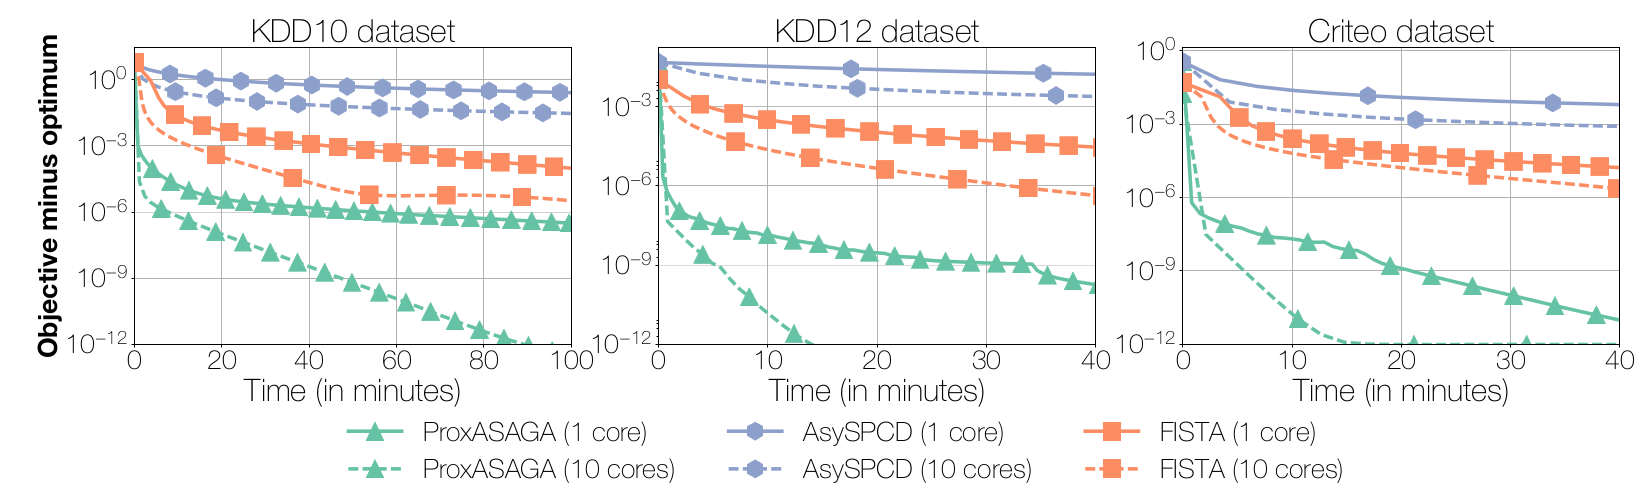
\includegraphics[width=1\linewidth]{img/prox_asaga_1}
% \end{column}%
% \end{columns}

ProxASAGA vs competing methods on 3 large-scale datasets, $\ell_1$-regularized logistic regression

\vspace{0em}\begingroup
\fontsize{9pt}{10pt}\selectfont
\begin{table}
\centering
%\resizebox{\linewidth}{!}{
\begin{tabular}{lrrrrr}
\toprule
{\bfseries\sffamily Dataset} & \multicolumn{1}{c}{$n$} & \multicolumn{1}{c}{$p$} & {{density}} & \multicolumn{1}{c}{$L$} & $\Delta$\\
\midrule
{\bfseries\sffamily KDD 2010} & \hfill 19,264,097 & \hfill 1,163,024 & \hfill $10^{-6}$ & \hfill 28.12 & 0.15\\
{\bfseries\sffamily KDD 2012} & \hfill 149,639,105 & \hfill 54,686,452 & \hfill $2 \times 10^{-7}$ & \hfill $1.25$ & 0.85\\
{\bfseries\sffamily Criteo} & \hfill 45,840,617 & \hfill 1,000,000 & \hfill $4 \times 10^{-5}$ & \hfill $1.25$ & 0.89\\
\bottomrule
\end{tabular}
%}
%\vspace{-5mm}
\end{table}
\endgroup


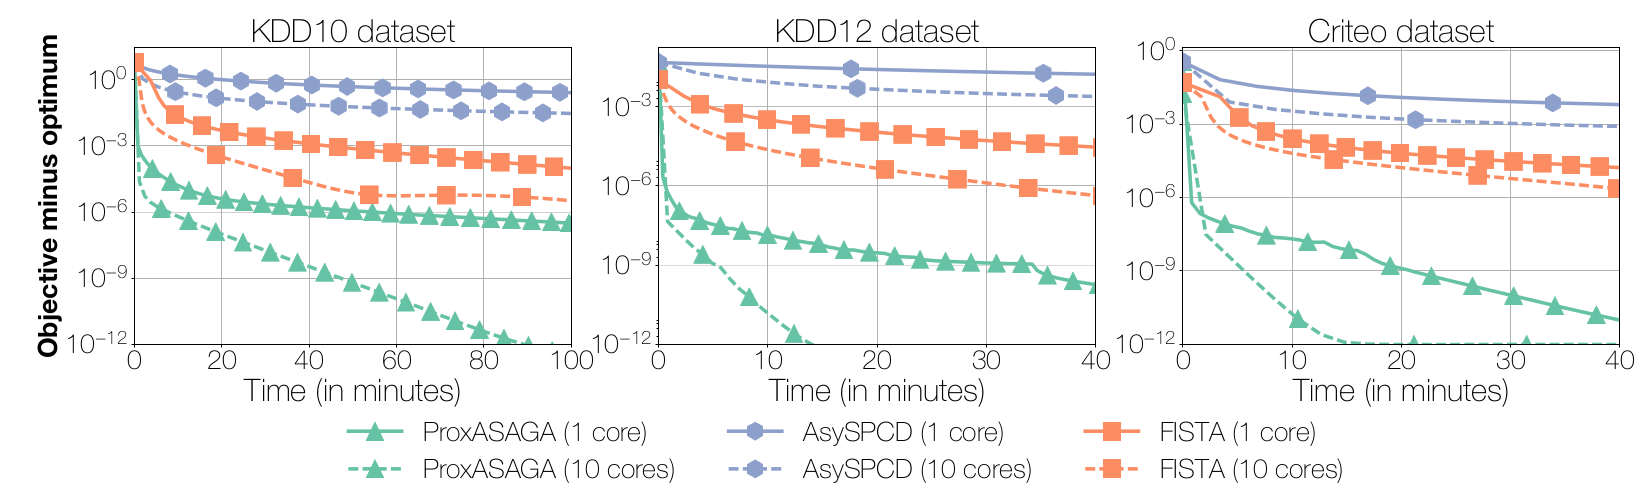
\includegraphics[width=1\linewidth]{img/prox_asaga_1}

\end{frame}


\begin{frame}{Empirical results - Speedup}

$$
\text{Speedup} = \frac{\text{Time to $10^{-10}$ suboptimality 
on one core}}{\text{Time to same suboptimality on $k$ cores}}
$$

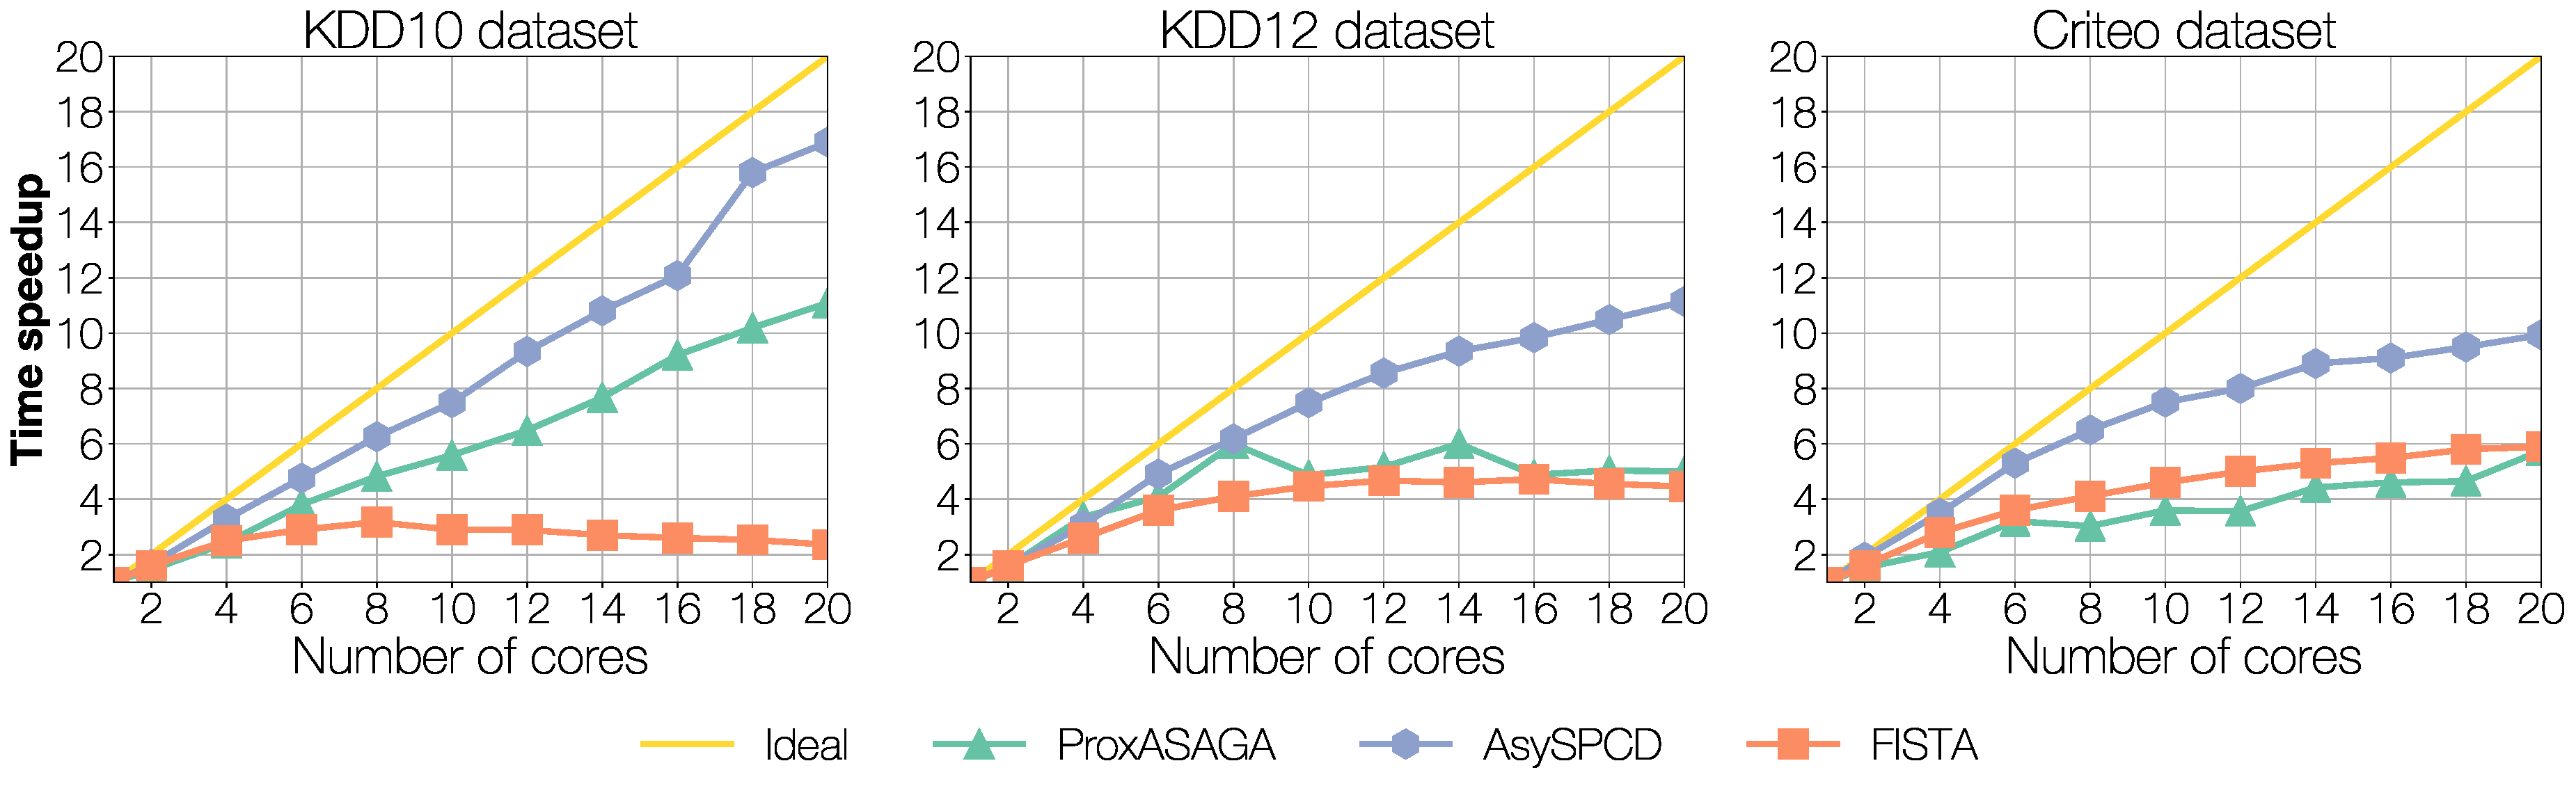
\includegraphics[width=\linewidth]{img/prox_asaga_2}

\begin{itemize}
\pause \item ProxASAGA achieves speedups between 6x and 12x on a 20 cores architecture.

\pause \vspace{0.5em}\item As predicted by theory, there is a high correlation between degree of sparsity and speedup.
\end{itemize}

\pause Thanks for your attention, see you at {\bfseries poster \#159}.
\end{frame}
% 
% \begin{frame}{References}
% \cite{pedregosa20016three}.
% \bibliographystyle{apalike}
% \printbibliography
% \end{frame}



% 
% \begin{frame}[fragile]{Generalization}
% This approach can be naturally generalized to $K$ classes.
% \begin{align}
% \Pr(Y_i=1) &= \frac{e^{\boldsymbol\beta_1 \cdot \mathbf{X}_i}}{1 + \sum_{k=1}^{K-1} e^{\boldsymbol\beta_k \cdot \mathbf{X}_i}} \nonumber \\
% \Pr(Y_i=2) &= \frac{e^{\boldsymbol\beta_2 \cdot \mathbf{X}_i}}{1 + \sum_{k=1}^{K-1} e^{\boldsymbol\beta_k \cdot \mathbf{X}_i}} \\
% \cdots & \cdots \\
% \Pr(Y_i=K-1) &= \frac{e^{\boldsymbol\beta_{K-1} \cdot \mathbf{X}_i}}{1 + \sum_{k=1}^{K-1} e^{\boldsymbol\beta_k \cdot \mathbf{X}_i}}
% \end{align}
% \end{frame}
% 
% 
% \begin{frame}[fragile]{Application}
% Lets use this to predict the future!
% 
% \pause
% Use the data from the religion dataset to predict how religious beliefs will evolve after 2017
% 
% \includegraphics[width=0.5\linewidth]{figures/religion.png}
% 
% \pause
% Suggestion: use scikit-learn's LogisticRegression class with {multi\_class='multinomial'}. Use as features the year and cohort. The model can predict probabilities with method predict\_proba.
% 
% \end{frame}
% 
% 
% 
% \begin{frame}[fragile]{Application}
% 
% 
% To predict, use the same data but with year and cohort shifted accordingly.
% 
% \includegraphics[width=0.5\linewidth]{figures/logistic_future.png}
% 
% 
% 
% \end{frame}
% 
% 
% 
\begin{frame}[noframenumbering, allowframebreaks]
\nocite{pedregosa2017proxasaga}
  % \frametitle{References}
  \printbibliography
 \end{frame}

\end{document}
